\documentclass[11pt,a4paper]{article}
\usepackage[margin=2.3cm]{geometry}
\usepackage{graphicx}
\usepackage{booktabs}
\usepackage{xcolor}
\usepackage[framemethod=tikz]{mdframed}
\usepackage{enumitem}
\usepackage{amsmath,amssymb}
\usepackage{hyperref}
\graphicspath{{figures/}}
\definecolor{good}{RGB}{34,139,84}
\definecolor{bad}{RGB}{190,40,40}
\definecolor{ink}{RGB}{40,80,160}
\newmdenv[backgroundcolor=blue!4,linecolor=ink,linewidth=1.2pt,roundcorner=6pt,innertopmargin=7pt,innerbottommargin=7pt]{notebox}
\newmdenv[backgroundcolor=green!5,linecolor=good,linewidth=1.2pt,roundcorner=6pt,innertopmargin=7pt,innerbottommargin=7pt]{goodbox}
\newmdenv[backgroundcolor=red!4,linecolor=bad,linewidth=1.2pt,roundcorner=6pt,innertopmargin=7pt,innerbottommargin=7pt]{badbox}
\setlength{\parskip}{5pt}
\hypersetup{colorlinks=true,linkcolor=ink,urlcolor=ink}
\newcommand{\astra}{GPT-6 Astra}
\title{\LARGE Physics-Faithful Engineering Drawings from \astra\\[4pt]\large An overview of what the model gets right, where it fails, and why that defines our work}
\author{SVG Patch Lab}
\date{12 September 2026}

\begin{document}
\maketitle

\begin{notebox}
\textbf{Summary.} We tested whether a frontier language model (\astra) can produce engineering drawings whose \emph{physics} is true --- not just whether the drawings look right. Across three rounds and 46 prompts it drafted flawlessly, computed every textbook result correctly, and --- unexpectedly --- drew heat, flow and torsion fields on irregular shapes that match our own numerical solver to within measurement noise. It failed on exactly three kinds of problem: boundaries that exchange heat with their surroundings (it exhausted its reasoning budget and produced nothing), fields that extend into open space (it drew a physically impossible picture without warning), and stress inside a loaded part (it painted a plausible map and admitted it was not a solution). Those three classes, and the silent-failure risk they expose, are the problems our solver-in-the-loop work has to address.
\end{notebox}

\section{What we are trying to do}
An engineering drawing is a set of claims. ``This beam's largest bending moment is 16\,kN$\cdot$m.'' ``The 40\,$^{\circ}$C isotherm passes here.'' ``Stress concentrates at this fillet.'' People build things from those claims. A drawing that states them wrongly is worse than no drawing, because it looks finished.

Drawings in SVG are made of instructions --- ``circle here, line there, text `200 mm' beside it'' --- so a language model can write them, and a program can read them back and check them. SVG Patch Lab already has the machinery for the second part: a strict parser, node identifiers, a patch format that protects geometry the model must not touch, and rendering-based metrics.

The question this study answers is:
\begin{notebox}
\textbf{When a language model draws an engineering picture, is the physics in it true? For which kinds of problem? And when it is not true, does the drawing say so?}
\end{notebox}
We consider a drawing \emph{physics-faithful} when four things hold: it is a valid, convention-correct drawing; every number it labels matches the true value within 2\,\%; every curve it declares to be a level set (an isotherm, a streamline, a stress contour) really lies where the field has that value; and where it cannot meet those conditions, it discloses that.

\section{How we tested}
\paragraph{Three rounds of increasing difficulty.}
\begin{itemize}[leftmargin=2em,itemsep=2pt]
  \item \textbf{Round 1 --- drafting (20 prompts).} Pure drawing tasks: flanges, gears, three-view projections, P\&IDs, schematics, floor plans. No physics to compute.
  \item \textbf{Round 2 --- computed physics (20 prompts).} Each drawing must carry results the model has to calculate: beam deflection, conduction through a composite wall, stress around a hole, member forces in a truss, Mohr's circle, natural frequencies, pipe flow, filter response, buckling loads, and so on. Four of the twenty are \emph{field} problems --- the answer is a whole map, not a number.
  \item \textbf{Round 3 --- fields with no formula (6 prompts).} Two-dimensional problems that can only be solved numerically: an L-shaped plate with a re-entrant corner, torsion of a square bar, a square annulus, flow through a sudden contraction, a square conductor in a round shell, and a plate losing heat through its edges.
\end{itemize}

\paragraph{Ground truth we computed ourselves.} Round-2 answers come from closed-form formulas evaluated by script, never typed by hand. Round-3 answers come from a finite-difference solver we wrote for the purpose; it reproduces the tabulated torsion constants of a square section to four significant figures, which is our check that the solver itself is right.

\paragraph{How we score a drawn curve.} Each Round-3 prompt fixes the mapping from physical coordinates to drawing coordinates and asks the model to tag every contour with its level. A script samples points along each drawn curve, maps them back to the physical domain, looks up our solver's field there, and records how far that value is from the curve's declared level. We call this the \textbf{field error} $\varepsilon$, in percentage points of the field's range. Our own solver's contours score about 0.05, which is the noise floor of the grid. A curve that is visibly in the wrong place scores several points; a wrong picture scores tens.

\section{Round 1: drafting}
\begin{center}
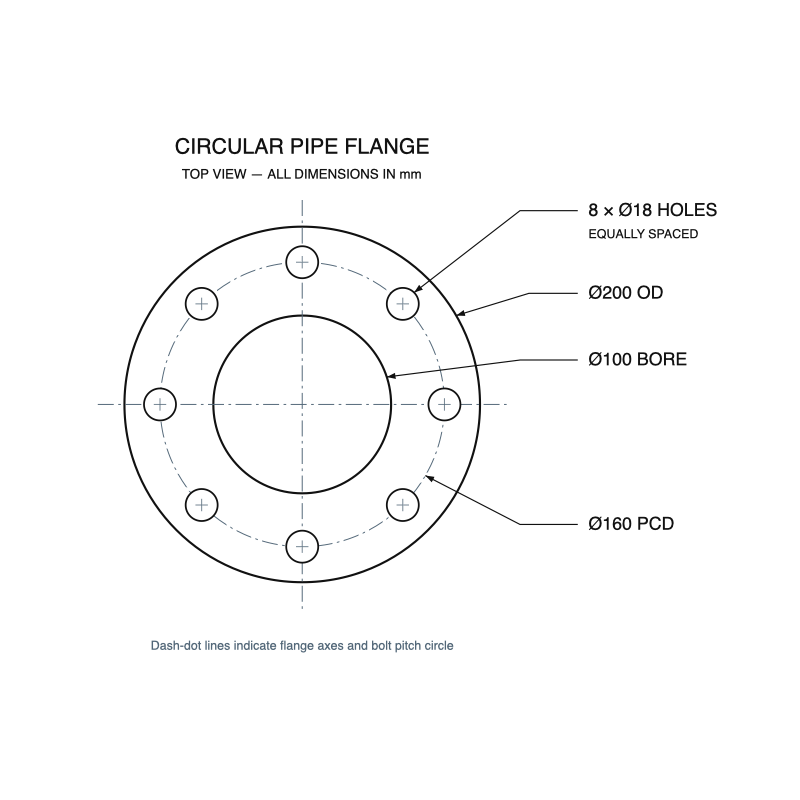
\includegraphics[width=0.44\textwidth]{flange.png}\hfill
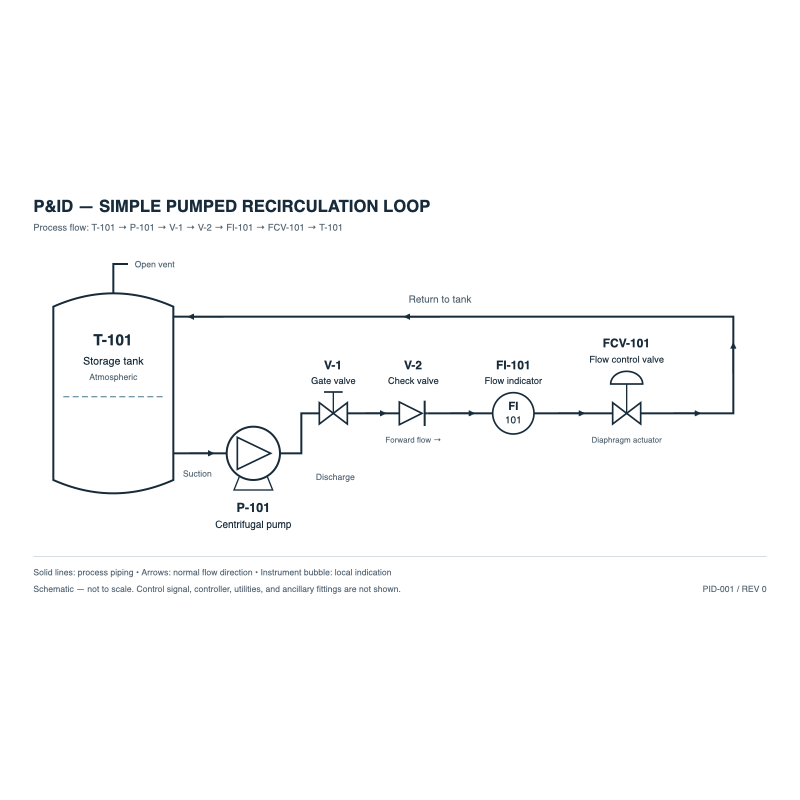
\includegraphics[width=0.52\textwidth]{pid.png}
\end{center}
\begin{goodbox}
\textbf{20 of 20 correct.} Every drawing parsed, rendered, and carried the required elements: eight holes on the pitch circle, dash-dot centrelines, hidden lines in the correct view, third-angle view placement, ISO~1219 valve envelopes with blocked centre ports, the ASME thread convention implemented as an SVG pattern, IEC terminal numbering on a motor starter, 14 risers and 13 treads on a stair section. Visual review found four minor convention slips: a pump drawn with the fluid-power symbol instead of the ISA one, a spring drawn as a rounded zigzag rather than a helix projection, a keyway with arrows but no numeral, and a shank diameter given as a note instead of a dimension. None affects what would be built.
\end{goodbox}

\section{Round 2: computed physics}
\begin{center}
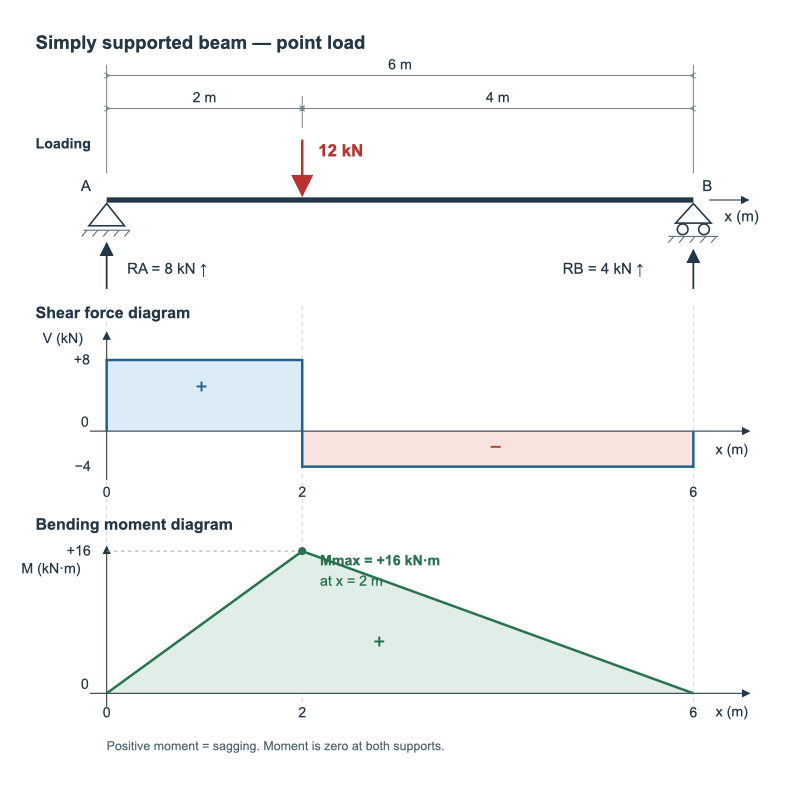
\includegraphics[width=0.50\textwidth]{beam.png}\hfill
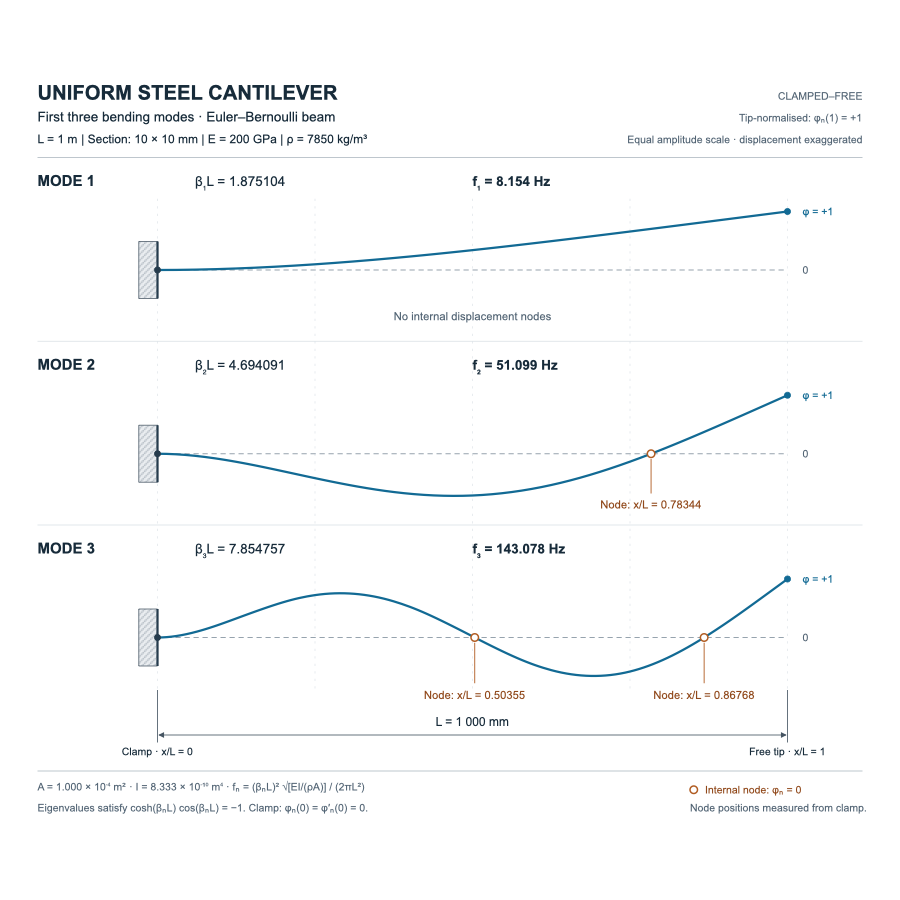
\includegraphics[width=0.46\textwidth]{modes.png}
\end{center}
\begin{goodbox}
\textbf{16 of 16 closed-form results correct}, typically to three or four significant figures: reactions of 8 and 4\,kN and a maximum moment of 16\,kN$\cdot$m for the loaded beam; heat flux and interface temperatures through a three-layer wall; the stress concentration factor of 3 at a hole; principal stresses and the principal angle from Mohr's circle; the cantilever eigenvalues $\beta L = 1.875,\ 4.694,\ 7.855$ with the resulting frequencies and the textbook node positions $x/L = 0.7834$ and $0.5035,\ 0.8677$; the fin parameter, tip temperature and efficiency; the Euler critical load; Lam\'e hoop stresses; shaft twist; the corner frequency, $-3$\,dB point and $-45^{\circ}$ phase of an RC filter.

The one item our checker flagged was our mistake, not the model's: we had written the bracket's section modulus with the wrong width. The model's 122\,MPa was right.

The model also noticed that one of our prompts was internally inconsistent (a Warren truss whose stated panel length and height cannot both be true for equilateral triangles) and wrote a note on the drawing explaining the discrepancy instead of silently choosing one.
\end{goodbox}

\paragraph{Two of the four field problems have analytic solutions, and the model reproduced them exactly.} For a square plate with one hot edge, the isotherm positions match the Fourier-series solution to three decimal places at every point we sampled (Fig.~\ref{fig:square}). For potential flow past a cylinder, the stream function is constant along every drawn streamline to within 1\,\%. The other two field problems have no formula, and they are where the failures begin (Section~\ref{sec:fail}).

\begin{figure}[h]
\centering
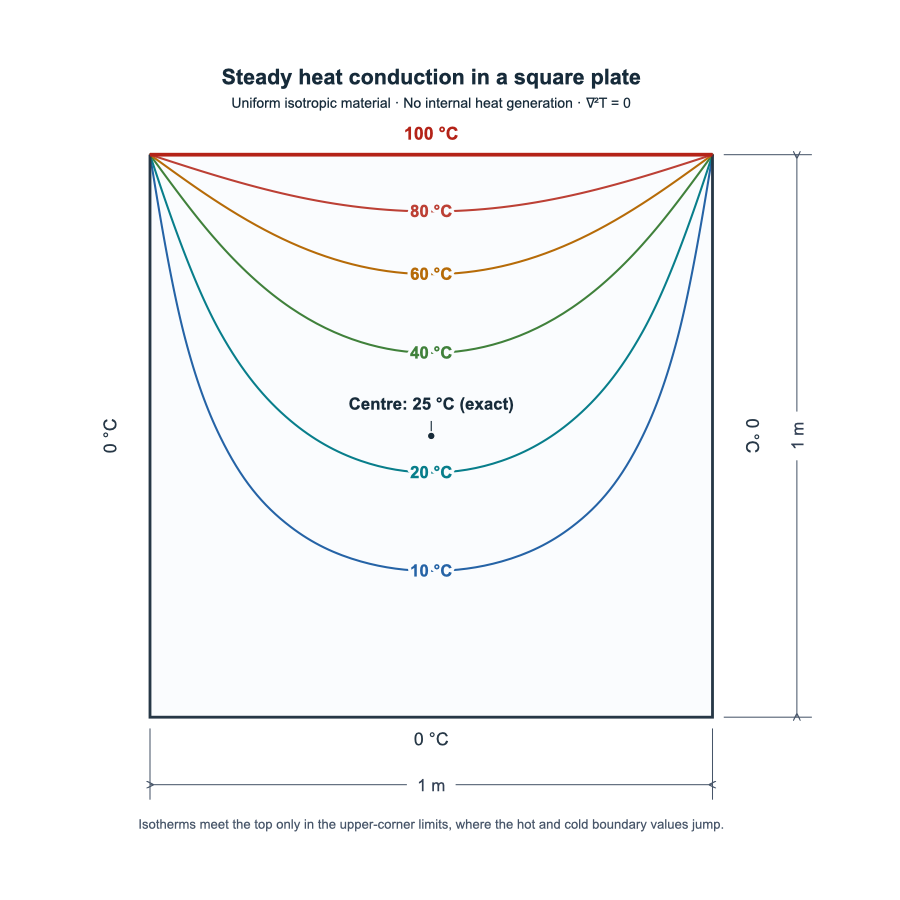
\includegraphics[width=0.46\textwidth]{laplace_square.png}
\caption{Round 2: isotherms in a square plate. Every knot lies on the series solution; the centre is exactly 25\,$^{\circ}$C.}
\label{fig:square}
\end{figure}

\section{Round 3: fields with no formula}
This round targeted exactly the class we expected to break: problems whose answer can only be obtained by solving a partial differential equation numerically. Figure~\ref{fig:overlay} shows the model's drawings with our finite-difference contours overlaid as red dashes.

\begin{figure}[p]
\centering
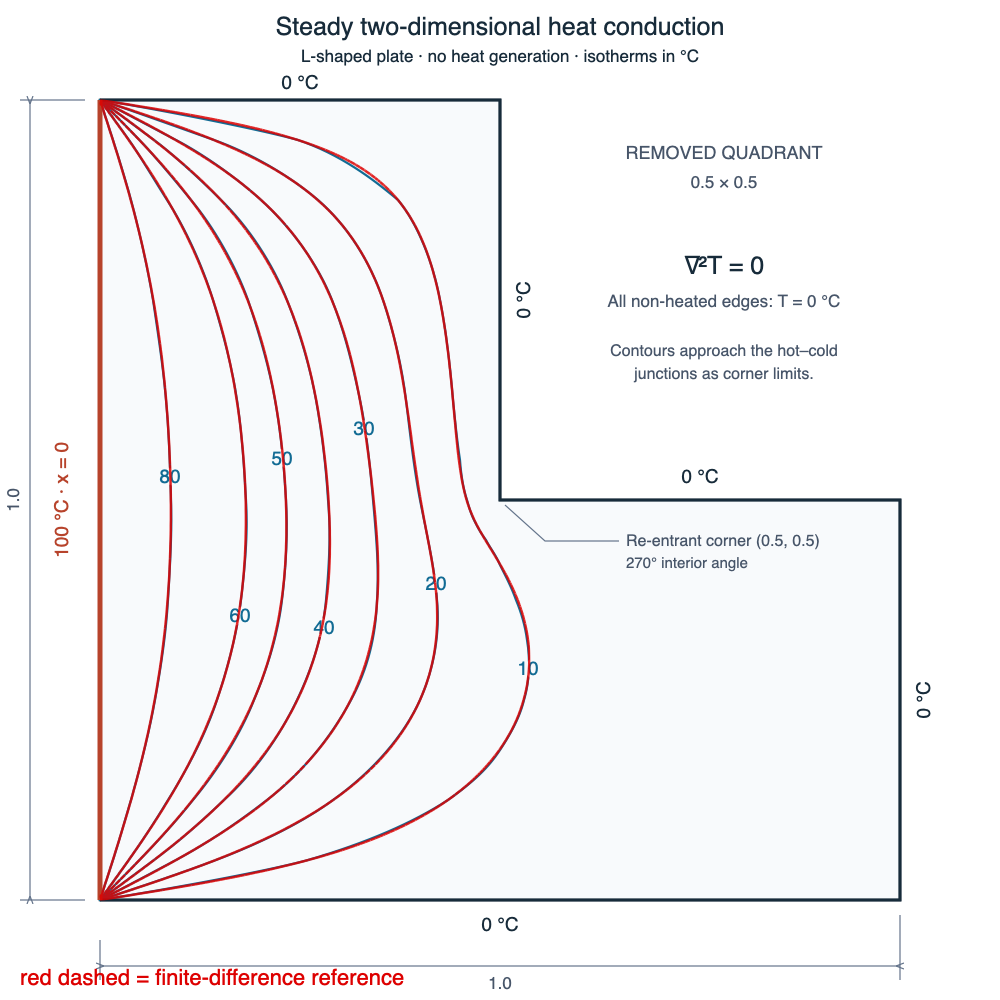
\includegraphics[width=0.47\textwidth]{lshape_overlay.png}\hfill
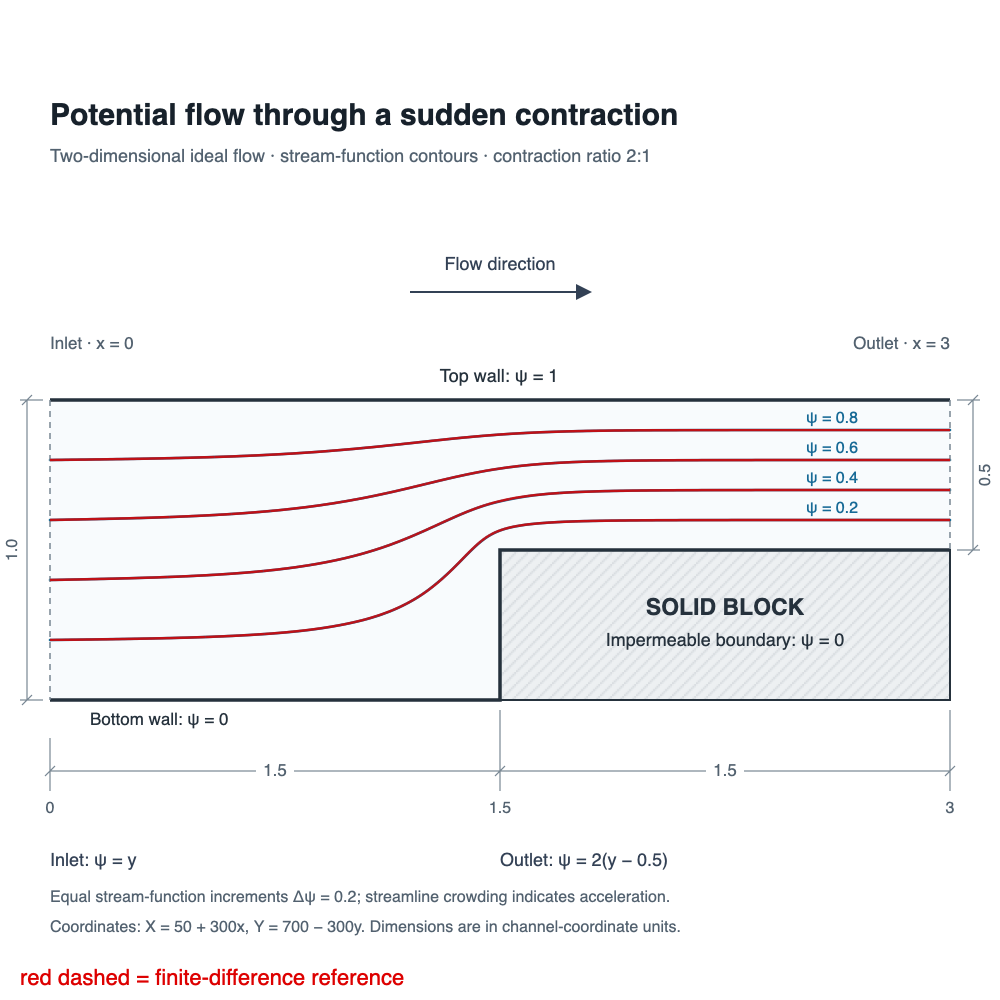
\includegraphics[width=0.50\textwidth]{channel_overlay.png}\\[10pt]
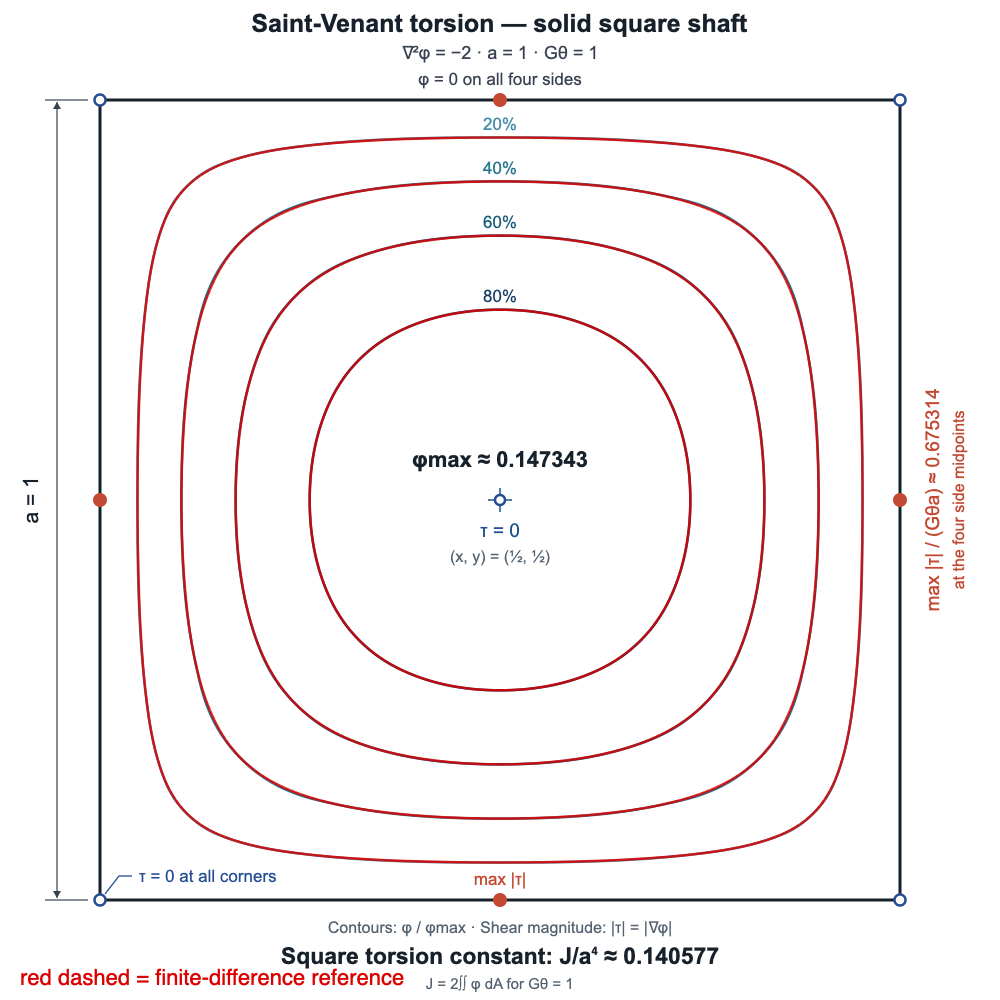
\includegraphics[width=0.47\textwidth]{torsion_overlay.png}
\caption{Round 3 overlays. Red dashes are the finite-difference reference. Top left: heat conduction in an L-shaped plate --- note the crowding at the re-entrant corner, which the model reproduced. Top right: streamlines through a 2:1 contraction. Bottom: the Prandtl stress function for torsion of a square bar; the model's $\phi_{\max}=0.147343$ and $J/a^4=0.140577$ match the reference to four figures.}
\label{fig:overlay}
\end{figure}

\begin{table}[h]
\centering\small
\begin{tabular}{p{5.2cm}p{3.4cm}rp{5.2cm}}
\toprule
Problem & Boundary type & $\varepsilon$ & Outcome \\
\midrule
Heat conduction, L-shaped plate & fixed temperatures & 0.13 & exact, including the corner singularity \\
Torsion of a square bar & fixed (zero) & 0.10 & exact \\
Square plate with square hole & fixed temperatures & 0.10 & exact \\
Flow through a sudden contraction & fixed stream function & 0.00 & exact \\
Square conductor in round shell & fixed potentials & 0.20 & exact \\
\midrule
Plate with \textbf{convective} edges & heat exchange with surroundings & --- & \textbf{no drawing produced} \\
\bottomrule
\end{tabular}
\caption{Field error $\varepsilon$ (percentage points of field range; the reference's own contours score $\approx0.05$).}
\label{tab:eps}
\end{table}

\begin{goodbox}
\textbf{Five of the six were solved, not sketched.} The drawn contours coincide with the reference within the grid's own noise. This was not expected: nothing in these problems can be looked up. How the model achieves it is an open question --- the reasoning budget it used (5{,}000--12{,}000 tokens) is far too small for a step-by-step relaxation over ten thousand grid points, so it is either exploiting structure (symmetry, conformal maps, series) or has some internal means of numerical computation. Either way, for two-dimensional Laplace and Poisson problems whose boundaries carry \emph{fixed values}, the model's fields are as good as a solver's.
\end{goodbox}

\section{Where it fails}\label{sec:fail}
The three failures are different in kind, and each calls for a different response.

\begin{badbox}
\textbf{Failure 1 --- exhausted reasoning, no output (convective boundary).}\\
The one Round-3 problem with a \emph{Robin} boundary --- edges that lose heat to the surrounding air in proportion to their temperature, rather than being held at a fixed value --- consumed the entire 16{,}000-token reasoning allowance and returned nothing. Not a wrong drawing: an empty response with a ``length'' stop reason. Whether a larger budget would rescue it is an open test. Every real heat-transfer problem has boundaries like this.
\end{badbox}

\begin{badbox}
\textbf{Failure 2 --- physically impossible, and undisclosed (field in open space).}\\
Asked for the electric field around two finite charged plates, the model drew the uniform region correctly (10\,kV/m) and then drew the fringing field at the plate ends as \emph{closed circular field lines}, with the outer equipotentials running off to infinity. Electrostatic field lines cannot form closed loops (the field has zero curl); the equipotentials must close around their conductor. The picture is convincing, passes every structural and numeric check we have, and carries no caveat beyond ``end contours schematic''. This is the most dangerous failure mode we observed.
\begin{center}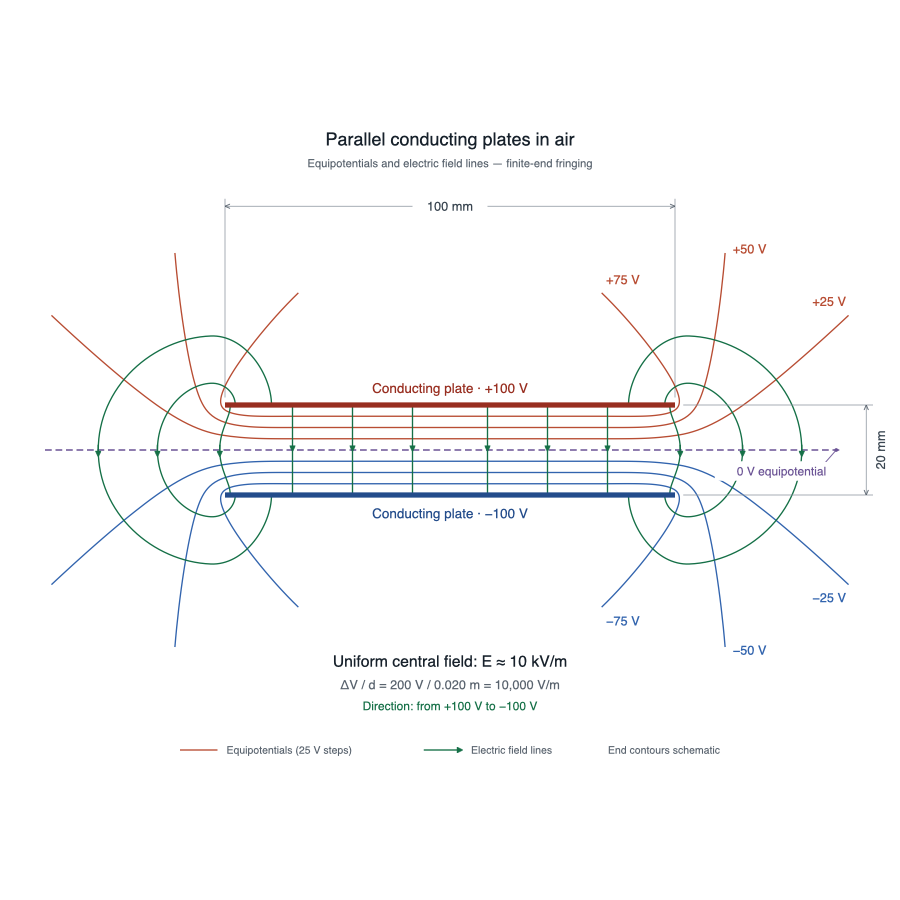
\includegraphics[width=0.55\textwidth]{capacitor.png}\end{center}
\end{badbox}

\begin{badbox}
\textbf{Failure 3 --- decorative, but disclosed (stress inside a part).}\\
Asked for the von Mises stress map of a loaded bracket, the model computed the scalar it could (the beam-theory root stress, correctly), painted an FEA-styled colour field with a hotspot at the inner corner, and labelled it ``illustrative --- not a solved FE model'' with an assumed concentration factor. The disclosure is exactly right; the field is not a solution and cannot tell an engineer where the part will crack.
\begin{center}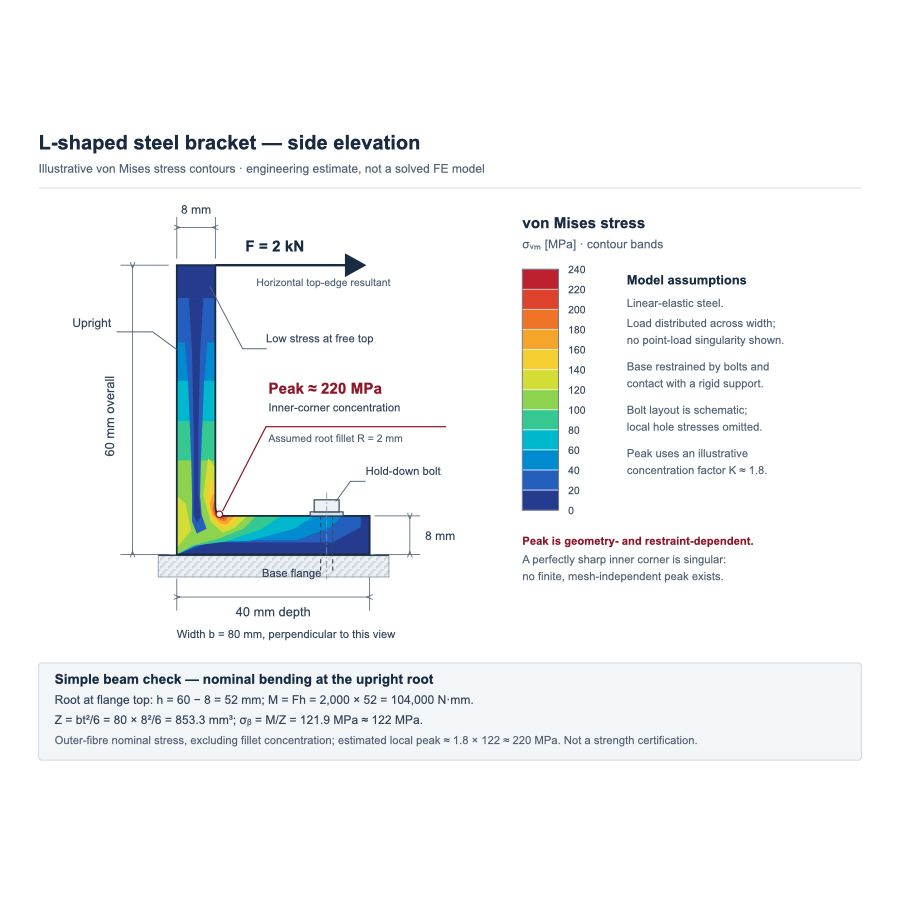
\includegraphics[width=0.55\textwidth]{bracket.png}\end{center}
\end{badbox}

\paragraph{Two lessons about checking, not about the model.} A structural check once flagged a correct gear because the model encoded the pitch circle as a path arc rather than a circle element; a contour scorer once reported a huge error because the model had drawn the torsion contours inside a translated group and the scorer ignored the transform. Both were false alarms, both fixed. Verification has to be geometric --- where is the curve, what is the field there --- not syntactic.

\section{Why this is our concern}
\begin{enumerate}[leftmargin=2em,itemsep=3pt]
  \item \textbf{Silent failure exists.} Failure~2 shows the model can hand over a physically impossible field with no warning. Drafting checks, numeric checks and a glance all pass. Only a solver-based comparison catches it.
  \item \textbf{The failing classes are the important ones.} Convective boundaries, open domains and stress fields are the everyday content of thermal and structural engineering. The model's strengths --- drafting and fixed-boundary potentials --- are real but do not cover them.
  \item \textbf{``Looks right'' had no number until now.} The field error $\varepsilon$ turns a judgement into a measurement: 0.1 for the solved cases, undefined-because-impossible for the capacitor. That metric, and the solver behind it, are the core of what we bring.
  \item \textbf{Disclosure is unreliable.} One failure disclosed itself; one did not. A system that ships model-drawn physics needs its own disclosure policy, not the model's.
\end{enumerate}

\section{What we propose to do}
Split the work along the line the data draws.
\begin{notebox}
\begin{itemize}[leftmargin=1.6em,itemsep=3pt]
  \item \textbf{The model drafts.} Layout, symbols, views, dimensions, leaders, legends, labels --- and the closed-form results it demonstrably gets right. This is where it is excellent.
  \item \textbf{A solver computes the fields the model cannot.} Convective and mixed boundaries, open domains, elasticity and stress, transient and nonlinear problems, real material data. The SVG supplies the geometry and boundary conditions; a finite-element solver (or a physics-informed network, where a parametric family or an inverse problem justifies it) returns the field.
  \item \textbf{The field re-enters the drawing as protected geometry.} Level sets are written into the SVG as tagged paths the model may label and lay out but may not alter or invent. This uses the patch-and-protect mechanism SVG Patch Lab already has.
  \item \textbf{Every field curve is verified before release.} The same scorer used in Round~3 compares the finished drawing against the solver. A drawing that fails is rejected; anything the model drew unaided is either verified or marked as unverified.
\end{itemize}
\end{notebox}

\section{Open questions}
\begin{itemize}[leftmargin=2em,itemsep=2pt]
  \item Does the fixed-boundary success survive arbitrary geometry --- random polygons, several holes --- or does it depend on structure the model can exploit?
  \item Is the convective-boundary failure a capability limit or a budget limit? A larger reasoning allowance settles it.
  \item Are stress fields always decorative? Plates with edge holes, interacting holes and filleted brackets, each with a finite-element reference, will measure this.
  \item Does putting the solver in the loop restore field fidelity without degrading drafting quality?
  \item How often does the model disclose a field it did not solve? The preliminary count is one in two.
\end{itemize}

\vfill
\begin{footnotesize}
\begingroup\raggedright
\noindent\textbf{Technical companions.} \texttt{astra\_failure\_analysis.pdf} (Round 1 in full), \texttt{astra\_physics\_analysis.pdf} (Round 2 in full), \texttt{astra\_proposal.pdf} (research proposal with hypotheses, work packages and evaluation plan). Model: OpenAI \texttt{gpt-6-astra}; harness and solvers in \texttt{scripts/}; prompt sets in \texttt{configs/prompts/}; all outputs and overlays in \texttt{runs/}.\par
\endgroup
\end{footnotesize}
\end{document}
